\section{Relativistic Mass Distribution}
\begin{quotation}
	\raggedleft \it The probability of them visiting is directly proportional\\ to how much you feel like being left alone \\
-- Einstein's Theory of Relatives
\end{quotation}
In the previous section, a Newtonian description for the fermion ball mass distribution was outlined. When large
masses are involved in calculations, it is often advisable to confirm the results with a relativistic treatment \cite{ref_bilic}, and
that is what this section will serve to provide. We choose to use units such that the speed of light and gravitational constant
are unity ($c=G=1$) and begin by assuming spherical symmetry of the fermion ball and a static solution, allowing the use of the
Schwarzschild metric
\begin{equation}
	ds^2=e^{\nu(r)}dt^2 - e^{\lambda(r)}dr^2 - r^2d\theta^2 - r^2 \sin^2\theta d\phi^2
	\label{eqn_schwarzschild}
\end{equation}
Using Einstein's field equations we obtain
\begin{equation}
	-8 \pi T_{\mu \nu} = R _{\mu \nu} - \frac{1}{2} R g_{\mu \nu} + \Lambda g_{\mu \nu}
	\label{eqn_einstein}
\end{equation}
The solutions to the field equations \cite{ref_tolmanpaper} are
\begin{eqnarray}
	&& 8 \pi T_0^0 = e^{- \lambda} \left(\frac{\lambda'}{r} - \frac{1}{r^2} \right) + \frac{1}{r^2} - \Lambda
	\label{eqn_einsteinsoln1} \\
	&& 8 \pi T_1^1 = - e^{- \lambda} \left(\frac{1}{r^2} - \frac{\nu'}{r} \right) + \frac{1}{r^2} - \Lambda
	\label{eqn_einsteinsoln2} \\
	&& 8 \pi T_2^2 = 8 \pi T_3^3 = \frac{e^{- \lambda}}{2} \left(\nu'' + \frac{\nu'^2}{2} + \frac{\nu'}{r} - \frac{\lambda'\nu'}{2}
	-\frac{\lambda'}{r} \right)
	\label{eqn_einsteinsoln3}
\end{eqnarray}
The approach to solving the relativistic mass distribution is to first solve the equation of hydrostatic equilibrium, interior and
exterior to the fermion ball and then to introduce the relativistic equation of state for a Fermi gas.

\subsection{Hydrostatic Equilibrium}
The fermion ball is treated as a perfect fluid \cite{ref_tolmanbook}
\begin{equation}
	T^{\mu \nu} = \frac{\partial x^\mu}{\partial x_0^\alpha} \frac{\partial x^\nu}{\partial x^\beta} T_0^{\alpha \beta}
	\label{eqn_relativisticfluid}
\end{equation}
which by definition is incapable of exerting transverse stress. Therefore the quantities of proper mass density $\rho_0(r)$
and proper hydrostatic pressure $P_0(r)$ may be defined as
\begin{eqnarray}
	&& T_0^{00} = \rho_0(r)
	\label{eqn_relativisticpropermassdensity} \\
	&& T_0^{11} = T_0^{22} = T_0^{33} = P_0(r)
	\label{eqn_relativisticproperpressure}
\end{eqnarray}
The only observable component of stress for a local observer will be the proper hydrostatic pressure. It follows that the
energy-momentum tensor becomes
\begin{equation}
	T^{\mu \nu} = \frac{\partial x^\mu}{\partial x_0^0}\frac{\partial x^\nu}{\partial x_0^0} \rho_0
		    + \frac{\partial x^\mu}{\partial x_0^1}\frac{\partial x^\nu}{\partial x_0^1} P_0
		    + \frac{\partial x^\mu}{\partial x_0^2}\frac{\partial x^\nu}{\partial x_0^2} P_0
		    + \frac{\partial x^\mu}{\partial x_0^3}\frac{\partial x^\nu}{\partial x_0^3} P_0
	\label{eqn_relativisticlocalpressure}
\end{equation}
where $x_0^0, x_0^1...$ are 'proper' coordinates and $x^0, x^1...$ are the points of interest. Also
\begin{equation}
	g^{\mu \nu} = \frac{\partial x^\mu}{\partial x_0^\alpha}\frac{\partial x^\nu}{\partial x_0^\beta} g_0^{\alpha \beta}
	\label{eqn_relativisticgnumu}
\end{equation}
reduces to
\begin{equation}
	\frac{d x^\mu}{ds} = \frac{\partial x^\mu}{\partial x_0^0}
	\label{eqn_relativisticgnumureduced}
\end{equation}
Inserting (\ref{eqn_relativisticgnumureduced}) into (\ref{eqn_relativisticlocalpressure}) gives
\begin{eqnarray}
	&T^{\mu \nu} =& (\rho_0 + P_0) \frac{dx^\mu}{ds} \frac{dx^\nu}{ds} - g^{\mu \nu} P_0 \nonumber \\
	\therefore \qquad &T_\mu^{\nu \phantom{\mu}} =& (\rho_0 + P_0) g_{\alpha \mu} \frac{dx^\alpha}{ds} \frac{dx^\nu}{ds} - g_\mu^\nu P_0
	\label{eqn_relativisticenergysoln}
\end{eqnarray}
In our static case we have
\begin{eqnarray}
	\frac{dt}{ds} &=& e^{-\frac{\nu}{2}}
	\label{eqn_relativisticstatic1} \\
	\frac{dr}{ds} &=& \frac{d\theta}{ds} = \frac{d\phi}{ds} = 0
	\label{eqn_relativisticstatic2}
\end{eqnarray}
which leads to
\begin{eqnarray}
	&& T_0^0 =  \rho_0
	\label{eqn_relativisticstatic3} \\
	&& T_1^1 =  T_2^2 = T_3^3 = -P_0
	\label{eqn_relativisticstatic4}
\end{eqnarray}
From (\ref{eqn_relativisticstatic4}), (\ref{eqn_einsteinsoln3}) and (\ref{eqn_einsteinsoln1}) we arrive at the relativistic
solution for hydrostatic equilibrium
\begin{equation}
	\frac{dP_0}{dr} + (\rho_0 + P_0) \frac{\nu'}{2} = 0
	\label{eqn_relativisticpressuredensitysolution}
\end{equation}
which is comparable to the Newtonian solution (\ref{eqn_hydroequil}).

\subsubsection{Exterior Solution (Schwarzschild)}
In empty space, all components of $T_\mu^\nu$ are zero. So by relating $T_0^0=T_1^1$ (\ref{eqn_einsteinsoln1}) and
(\ref{eqn_einsteinsoln2}), it is clear that $\lambda'=-\nu'$. Again, relating to $T_2^2$ (\ref{eqn_einsteinsoln3}) it follows
that
\begin{equation}
	\nu'' + \nu'^2 + \frac{2\nu'}{r} =0
	\label{eqn_relativisticarb1}
\end{equation}
which has a solution in the form
\begin{equation}
	e^\nu = a + \frac{b}{r}
	\label{eqn_relativisticarb2}
\end{equation}
Using the special relativity metric and restoring the correct units
\begin{equation}
	e^{-\lambda} = 1 - \frac{2 G M}{c^2 r}
	\label{eqn_relativisticarb3}
\end{equation}
where $M$ is the total mass.

\subsubsection{Interior Solution (Oppenheimer and Volkoff)}
This solution was originally formulated in \cite{ref_oppenheimervolkoff} as a means to explore the physics of massive neutron
cores. Due to the presence of the fermions, we can no longer make the equality between (\ref{eqn_einsteinsoln1}),
(\ref{eqn_einsteinsoln2}) and (\ref{eqn_einsteinsoln3}) as in the exterior solution, $T_\mu^\nu$ is now non-zero. By using a
trial and error approach and introducing a variable which has the form
\begin{equation}
	u(r) = \frac{r}{2}\left(1-e^{-\lambda}\right)
	\label{eqn_relativisticarb4}
\end{equation}
the $T_0^0$ solution (\ref{eqn_einsteinsoln1}) then becomes
\begin{equation}
	\frac{du}{dr} = 4 \pi \rho_0 r^2
	\label{eqn_relativisticarb5}
\end{equation}
At the outer radius ($R$, which must be continuous with the exterior solution), we see that
\begin{equation}
	u_R = \frac{R}{2}\left(1-e^{-\lambda(R)}\right) = M
	\label{eqn_relativisticarb6}
\end{equation}
So the solution to $e^{-\lambda}$ is the same for both the interior and the exterior (\ref{eqn_relativisticarb3}). Re-inserting the
correct units, $T_1^1$ (\ref{eqn_einsteinsoln2}) becomes
\begin{equation}
	\frac{dP_\nu}{dr} = - \frac{G}{r^2} \left(\frac{ \rho_0+ \frac{P_\nu}{c^2}}{r-2u}\right) \left( m + \frac{4 \pi P_\nu r^3}{c^2} \right)
	\label{eqn_relativisticarb7}
\end{equation}

\subsection{Equation of State for a Relativistic Degenerate Fermi Gas}
This is by far the simplest approach to derive the equation of state for a relativistic degenerate Fermi gas \cite{ref_chandra}.
We begin by confining $N$ fermions in a volume $V$. The number of quantum states with momentum between $p$ and $p+dp$ is given by
\begin{equation}
	\frac{4 V \pi g_\nu p^2 dp}{h^3}
	\label{eqn_chandra1}
\end{equation}
Pauli's exclusion principle implies
\begin{equation}
	N(p)dp \le \frac{4 V \pi g_\nu p^2 dp}{h^3}
	\label{eqn_chandra2}
\end{equation}
A completely degenerate gas has all lowest states occupied
\begin{equation}
	N(p) = \frac{4 V \pi g_\nu p^2}{h^3}
	\label{eqn_chandra3}
\end{equation}
If there is a finite number $N$ of fermions, then they must all have momentum less than the Fermi momentum $p_0$ such that
\begin{equation}
	N = \frac{4 V \pi g_\nu}{h^3} \int_0^{p_0}p^2dp = \frac{4 V \pi g_\nu p_0^3}{3 h^3}
	\label{eqn_chandra4}
\end{equation}
The Fermi momentum is related to number density by
\begin{equation}
	n = \frac{N}{V} = \frac{4 \pi g_\nu p_0^3}{3 h^3}
	\label{eqn_chandra5}
\end{equation}
The pressure is the mean rate of transfer of momentum across an ideal surface of unit area, from this we obtain
\begin{equation}
	PV=\frac{1}{3} \int_0^{\infty}N(p)pv_pdp
	\label{eqn_chandra6}
\end{equation}
where $v_p$ is the associated velocity, this leads to
\begin{equation}
	P=\frac{4\pi g_\nu}{3h^3} \int_0^{p_0}p^3\frac{\partial E}{\partial p}dp
	\label{eqn_chandra7}
\end{equation}
The internal energy of the gas (due to translational energy of the motions of individual fermions) is
\begin{equation}
	U=\int_0^\infty N(p) E dp
	\label{eqn_chandra8}
\end{equation}
for complete degeneracy we get
\begin{eqnarray}
	&&U=\frac{4V\pi g_\nu}{h^3} \int_0^{p_0} E p^2 dp
	\label{eqn_chandra9} \\
	\therefore &&P = \frac{4\pi g_\nu}{3h^3} E(p_0)p_0^3 - \frac{U}{V}
	\label{eqn_chandra10}
\end{eqnarray}
and according to special relativity
\begin{eqnarray}
	&&E = mc^2\left(\sqrt{1+\frac{p^2}{m_\nu^2 c^2}}-1\right)
	\label{eqn_chandra11} \\
	&&\frac{\partial E}{\partial p} = \frac{1}{m_\nu} \left( 1 + \frac{p^2}{m_\nu^2c^2}\right)^{-\frac{1}{2}} p
	\label{eqn_chandra12}
\end{eqnarray}
Inserting into (\ref{eqn_chandra7}) we arrive at
\begin{equation}
	P = \frac{4\pi g_\nu}{3 m_\nu h^3} \int_0^{p_0} \frac{p^4 dp}{\sqrt{1+\frac{p^2}{m_\nu^2 c^2}}}
	\label{eqn_chandra13}
\end{equation}
By substituting $\sinh \theta = \frac{p}{mc}$ we get
\begin{eqnarray}
	P &=& \frac{4\pi g_\nu m_\nu^4c^5}{3h^3} \int_0^{\theta_0} \sinh^4 \theta d\theta \nonumber \\
	  &=& \frac{4\pi g_\nu m_\nu^4c^5}{3h^3} \left[ \frac{\sinh^3\theta \cosh \theta}{4} -\frac{3 \sinh 2\theta}{16} + \frac{3\theta}{8} \right]_{\theta = \theta_0}
	\label{eqn_chandra14}
\end{eqnarray}
By making the following substitution, in order that we may use a more convenient unit in dealing with Fermi momentum
\begin{equation}
	X=\frac{p_0}{m_\nu c}
	\label{eqn_relatfermibetterunits}
\end{equation}
and using $\sinh^{-1}X=\ln(X+\sqrt{1+X^2})$, (\ref{eqn_chandra14}) reduces to
\begin{equation}
	P = K \left[ X\left(1+X^2\right)^{\frac{1}{2}}\left(\frac{2}{3}X^2-1\right) + \ln \left(X+\left(1+X^2\right)^{\frac{1}{2}}\right)\right]
	\label{eqn_chandra15}
\end{equation}
where
\begin{equation}
	K = \frac{g_\nu m_\nu^4 c^5}{16\pi^2\hbar^3}
	\label{eqn_chandra16}
\end{equation}
Noting that the mass energy density is given by the internal energy density plus the addition of all the fermion rest mass energies, we get
\begin{equation}
	\rho = \frac{U}{Vc^2} + nm
	\label{eqn_chandra17}
\end{equation}
Working from (\ref{eqn_chandra17}), (\ref{eqn_chandra10}) and (\ref{eqn_chandra5}) we obtain the relativistic equation of state for
a Fermi gas, concerning the proper mass density
\begin{equation}
	\rho = \frac{K}{c^2}\left[X\left(2X^2+1\right)\left(1+X^2\right)^{\frac{1}{2}} - \ln \left( X+\left( 1+X^2\right)^{\frac{1}{2}}\right) \right]
	\label{eqn_chandra18}
\end{equation}
Equations (\ref{eqn_chandra15}), (\ref{eqn_chandra16}) and (\ref{eqn_chandra18}) fulfil our requirements for the degenerate relativistic
equation of state for a Fermi gas.

\subsection{Mass Distribution}
\label{sec_relatmassdist}
Now that we have formulated the equation of hydrostatic equilibrium and the equation of state for a degenerate relativistic Fermi gas,
we may combine them in order to find the mass distribution of the fermion ball. By using the dimensionless units
\begin{equation}
	x=\frac{r}{b_\nu} \qquad \mu = \frac{m}{d_\nu}
	\label{eqn_relatmassdistunits}
\end{equation}
where
\begin{equation}
	b_\nu = \sqrt{\frac{4 \pi \hbar^3}{G g_\nu m_\nu^4 c}} \qquad d_\nu = 2\sqrt{\frac{4 \pi \hbar^3 c^3}{G^3 g_\nu m_\nu^4}}
	\label{eqn_relatdimensionless}
\end{equation}
It is possible to obtain the mass distribution from (\ref{eqn_relativisticarb7}), (\ref{eqn_chandra16}) and (\ref{eqn_chandra18}) by
integrating over the density as in the Newtonian solution (\ref{eqn_classicalmassintegral}).
\begin{align}
	\frac{dX}{dx} = - &\frac{1+X^2}{X\left(x^2 - 2\mu x\right)} \nonumber \\
			  &\left\{ \mu +x^3 \left[ X\left(1+X^2\right)^{\frac{1}{2}}
			  \left(\frac{2}{3}X^2-1\right) + \ln \left(X + \left( 1+X^2\right)^{\frac{1}{2}} \right)\right]\right\}
	\label{eqn_relativisticxsolution} \\
	\frac{d\mu}{dx} = x^2&\left\{ X\left( 1+X^2\right)^{\frac{1}{2}} \left(2X^2+1\right)
			  - \ln \left(X + \left( 1+X^2\right)^{\frac{1}{2}} \right)\right\}
	\label{eqn_relativisticmusolution}
\end{align}
And again, as in the Newtonian case, these equations must be solved numerically. As we have no
need for inserting a baryon core, we simply set $\mu(x_0)=0$ and select a value for the Fermi momentum $X(x_0)$. This allows for calculation
of the total mass and radius of the fermion ball from a single parameter (besides the fermion characteristics), but has the
disadvantage of requiring a trial and error technique when selecting total mass. Solutions for $X$, $\mu$ and $\mu'$ are presented in
Figure \ref{fig_relativisticsolution}.
\begin{figure}[!p]
	\begin{center}
	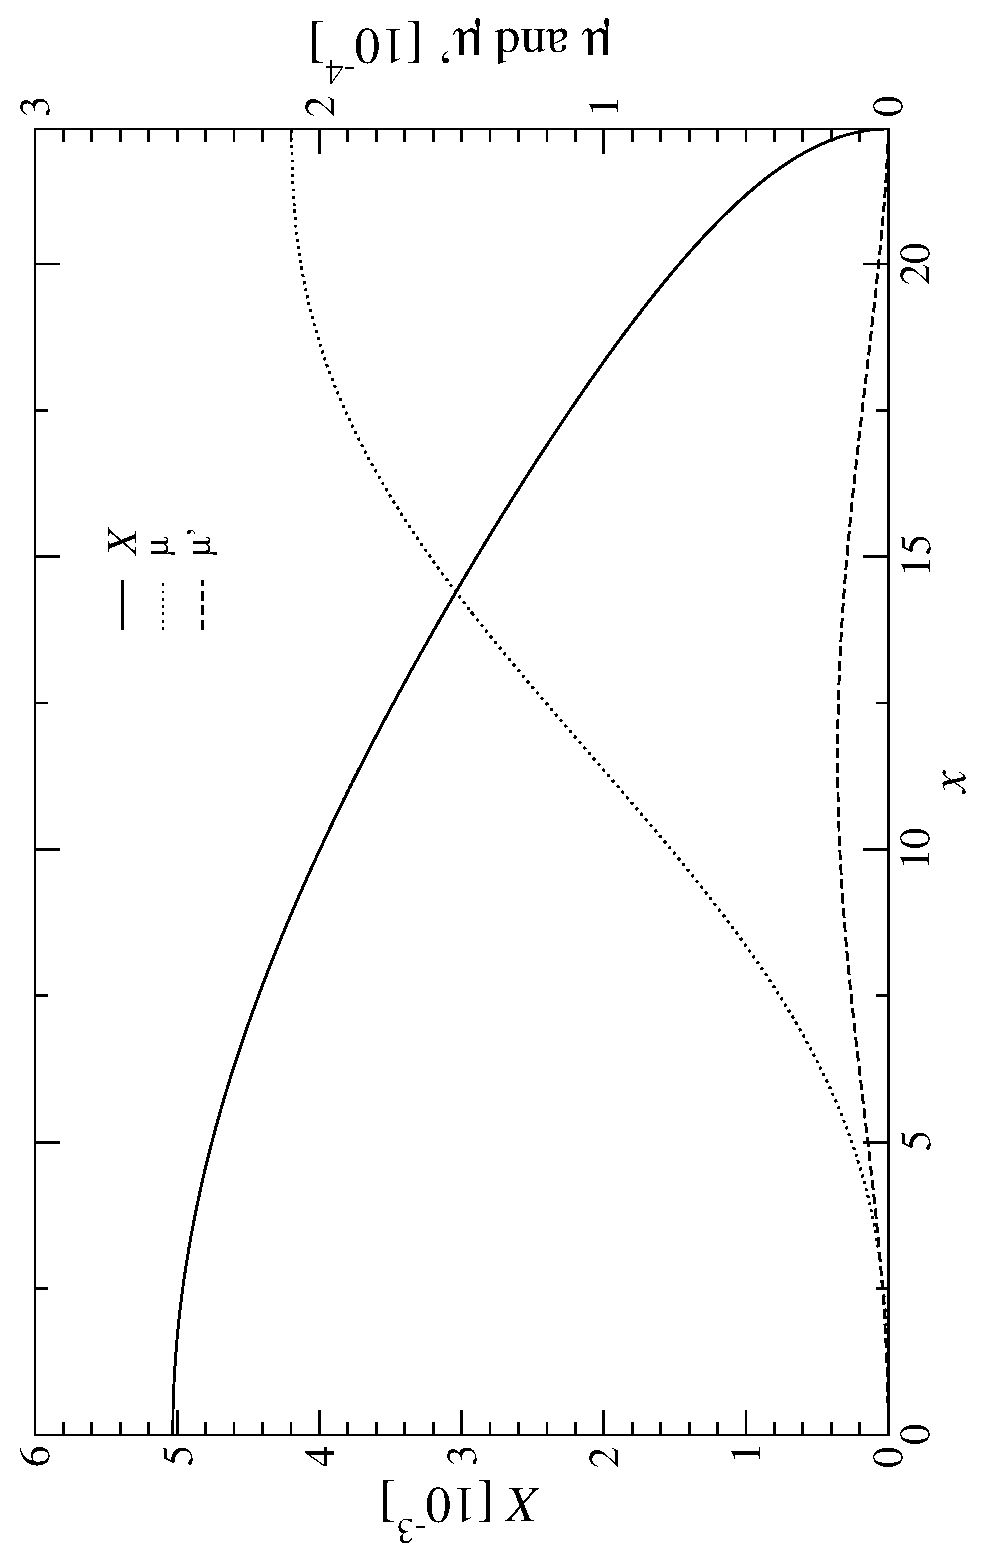
\includegraphics[angle=-90,width=0.9\textwidth]{eps/relativisticsolution.eps}
	\caption{Relativistic solution of the dimensionless mass $\mu$, derivative $\mu'$ and Fermi momentum $X$ as functions of the
	dimensionless radius.}
	\label{fig_relativisticsolution}
	\end{center}
\end{figure}

It is enlightening to find that the relativistic derivation of the mass distribution has confirmed the classical method.
For this reason, graphs of mass
distribution will not be shown as they are identical to those in Section \ref{sec_classical}. However, the relativistic approach has been
useful, as it has also revealed more information about the fermion ball. It is now possible to plot a relativistic relation
between total mass and radius (Figure \ref{fig_relativisticmvsr}) and has also given an alternative numerical technique for calculating
$M$ and $M'$, in fact this method turns out to be preferred in the spectra simulations of Section \ref{sec_accretion}.

It is clear from the mass-radius plot that the fermion ball is indeed non-relativistic, as relativistic
effects are only prevalent near the Oppenheimer-Volkoff limit, which is a factor of $10^3$ larger than the mass of the centre of our galaxy.
The Oppenheimer-Volkoff limit is the maximal mass which a degenerate fermion ball can have.
It is noteworthy that this Oppenheimer-Volkoff limit is very much comparable to the mass of the largest
observed super-massive, compact, dark object which is $3\times 10^9M_\odot$; M87 in the Virgo cluster \cite{ref_centralobjects}.
\begin{figure}[!p]
	\begin{center}
	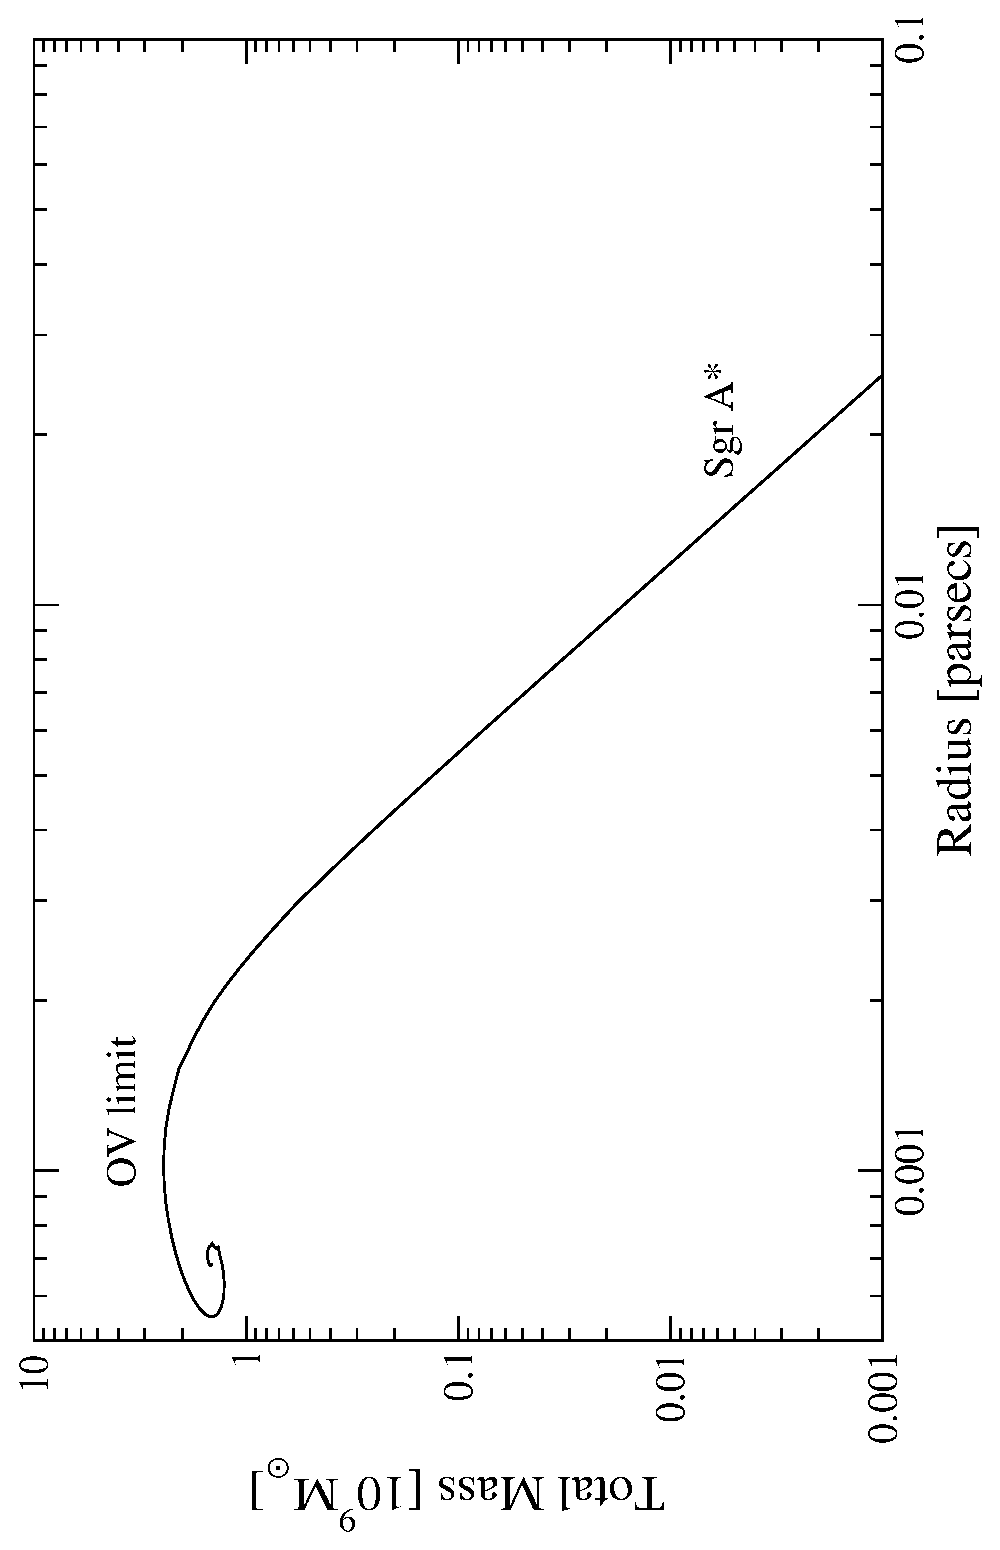
\includegraphics[angle=-90,width=0.9\textwidth]{eps/relativisticmvssr.eps}
	\caption{Relativistic mass-radius relation. Note the turning point is the Oppenheimer-Volkoff limit (2.45$\times 10^9 M_\odot$)
	and the curve left of the maximum represents unstable configurations curling around the point of infinite central density.
	The mass-radius region which the centre of our galaxy lies within is noted as Sgr A*. As previously decided upon, this
	is for 16keV, $g_\nu=2$ fermions.}
	\label{fig_relativisticmvsr}
	\end{center}
\end{figure}
